\section{Uppgift 2}\label{sec:uppg02}

\subsection{Instruktioner}
\begin{Verbatim}[fontsize=\small]
Skriv en klass Konto som representerar ett bankkonto. Klassen ska innehålla
data om ett bankkonto enligt följande (alltså klassens instansvariabler):

saldo (double)
kundnr (int)
kundnamn (String)

Klassen ska även ha en klassvariabel (static variabel) som heter:

räntesats (double)

Varför ska den vara en klassvariabel? Jo, eftersom alla konton har samma
räntesats (ränta per år).

De metoder som ska finnas i klassen Konto är följande:

- insättning, metod som ökar saldot med parameterns värde.
- uttag, metod som minskar saldot med parameterns värde.
- hämtaSaldo, metod som returnerar saldo.
- hämtaKundnamn, metod som returnerar kundnamn.
- avläsRänteSats, *klassmetod* som returnerar räntesatsen.

Det ska naturligtvis finnas en konstruktor.

Skriv en testklass (testprogram) som skapar två konton. Gör insättning och
uttag med valfria belopp på kontona. Skriv sedan ut kontonas saldon och kundens
namn. Skriv sist ut vilken räntesats de båda kontona har.
\end{Verbatim}


\subsection{Källkod}
\subsubsection{Lab4Uppg02.java}
\javacode{src/Lab4Uppg02.java}
\caption{Lab4Uppg02.java}
\label{src:uppg02}

\subsubsection{Konto.java}
\javacode{src/Konto.java}
\caption{Konto.java}
\label{src:konto}

% Screenshots med Bash, terminalfönsterstorlek 90x40
\subsection{Skärmdump}
Se Figur~\ref{fig:uppg02-screenshot} för skärmdump på körning av koden i
Sektion~\ref{src:uppg02} och Sektion~\ref{src:konto}.

\begin{figure}[htbp]
\centering
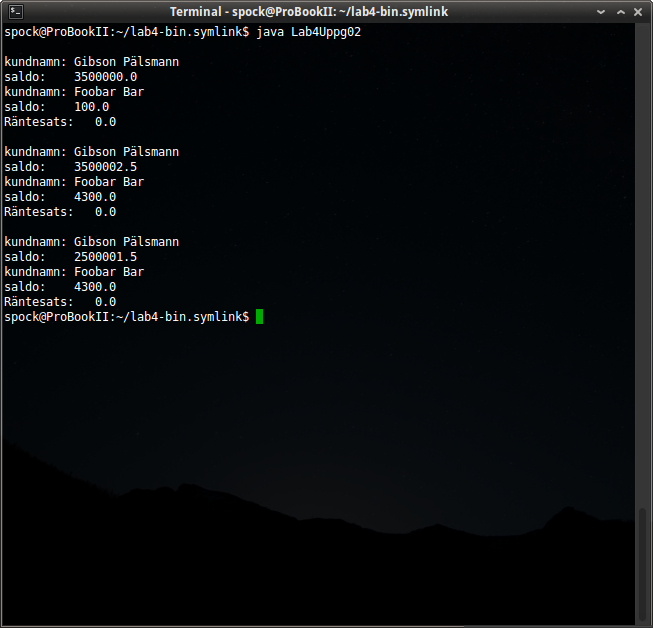
\includegraphics[width=\linewidth]{img/02.png}
\caption{Körning av koden till Uppgift~\ref{sec:uppg02}}
\label{fig:uppg02-screenshot}
\end{figure}

